\documentclass{alex_hü}

\name{Alexander Helbok}
\course{PS Physik}
\hwnumber{2}


\begin{document}
\renewcommand{\labelenumi}{\alph{enumi})}


\begin{mybox}{2. Feld einer Hohlkugel}
	\centering \( m = 5 \unit{kg};\quad k = 2 \unit{N/m};\quad a = 0.1 \unit{m};\quad h = 0.4 \unit{m};\quad l = 0.1 \unit{m} \)
	\tcblower
	\begin{enumerate}
		\item \( \rho = \tfrac{Q}{V} \)
		\begin{flalign*}
			V &= \int_V dV = \int\limits_{0}^{\pi}\int\limits_{0}^{2\pi}\int\limits_{R_i}^{R_a} r^2\sin(\theta)\ \mathrm{d}r\mathrm{d}\varphi\mathrm{d}\theta &&\\
			&= \tfrac{4}{3}\pi(R_a^3-R_i^3) &&\\
			\rho &= \dl{\tfrac{3Q}{4\pi} (R_a^3-R_i^3)} &&
		\end{flalign*}
	\tcbline
		\item \( F = -m\omega^2 x;\quad \Delta x = x_1 - x_2 \)
		\begin{flalign*}
			m\ddot{x_1} &= -m\omega_a\!^2x_1 - k(x_1 - x_2) &&\\
			m\ddot{x_2} &= -m\omega_a\!^2x_2 - k(x_2 - x_1) &&\\
			\Rightarrow\ m(\ddot{x_1}& - \ddot{x_2}) = -m\omega_a\!^2(x_1 - x_2) - 2k(x_1 - x_2) = -(m\omega_a\!^2 + 2k)(x_1 - x_2) &&\\
			\Delta \ddot{x} &= -\tikzmark{Startw} (\omega_a\!^2 + \tfrac{2k}{m}) \tikzmark{Endw} \Delta x &&\\[3.5ex]
			\omega_b &= \sqrt{\omega_a^2 + \tfrac{2k}{m}} = \dl{6.43 \unit{rad/s}} &&
		\end{flalign*}
		\AddUnderBrace{Startw}{Endw}{$= \omega_b$}
	\tcbline
		\item \( \delta\omega = \omega_b - \omega_a \)
		\begin{flalign*}
			0 &= \cos(\tfrac{1}{2}\delta\omega t) &&\\
			t &= \tfrac{2\arccos(0)}{\delta\omega} = \dl{50.29 \unit{s}} &&
		\end{flalign*}
	\end{enumerate}
\end{mybox}
\newpage
\begin{mybox}{3. Zwei ringförmige Ladungsträger}
	\centering \( k = \tfrac{1}{4\pi \epsilon_0} \)
	\tcblower
	\begin{enumerate}
		\item \(h = \sqrt{r^2+z^2};\quad \cos(\theta) = \tfrac{z}{h};\quad \mathrm{d}Q = \lambda \mathrm{d}r;\quad \mathrm{d}r = r \mathrm{d}\varphi;\quad Q = 2r\pi \lambda \)\\
		\begin{center}
		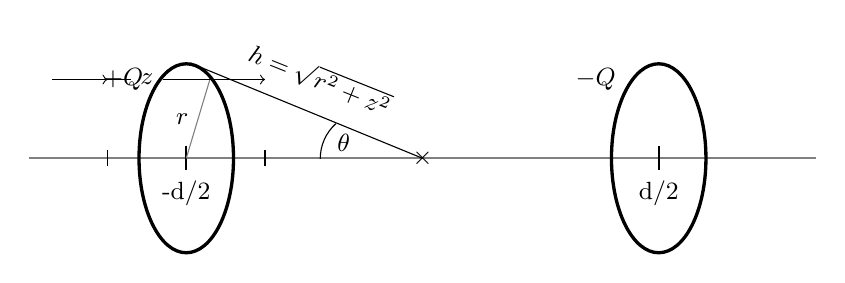
\begin{tikzpicture}
			\tikzmath{\x = 2; \y = -0.9;}
%			-------|--------|------
			\draw [gray, thick](0,0)--(10,0);
			\draw [thick] (2,-0.15)--(2,0.15) node [below, pos=0] {\small -d/2};
			\draw [thick] (8,-0.15)--(8,0.15) node [below, pos=0] {\small d/2};
			\node (c) at (5,0) {\small \( \times \)};
%			figures
			\draw [gray] (2,0)--(2.3,1) node [black, left, pos=0.5] {\small \( r \)};
			\draw (2.05,1.21)--(5,0);
			\node [rotate=-21.8] at (3.7,1) {\small \(h = \sqrt{r^2+z^2} \)};
			\draw (3.9, 0.44) arc (132:180:0.6);
			\node at (4, 0.2) {\small \( \theta \)};
			\draw [very thick] (2,0) ellipse (0.6 and 1.2);
			\node at (1.2,1) {\small \( +Q \)};
			\draw [very thick] (8,0) ellipse (0.6 and 1.2);
			\node at (7.2,1) {\small \( -Q \)};
%			<--- z ---->
			\draw (\x,\y-0.1)--(\x,\y+0.1);
			\draw (\x+3,\y-0.1)--(\x+3,\y+0.1);
			\node at (\x+1.5,\y) {\small{$ z $}};
			\draw [to-] (\x,\y) -- (\x+0.3,\y);
			\draw (\x+0.5,\y) -- (\x+1.3,\y);
			\draw [-to] (\x+1.7,\y) -- (\x+3,\y);
		\end{tikzpicture}\\[2ex]
		Due to the symmetric nature of this problem we can neglect vertical components of forces
		\end{center}	
		\begin{flalign*}
			\mathrm{d}E_1(z) &= k \tfrac{\mathrm{d}Q}{h^2} \cos(\theta) = k \tfrac{\lambda \mathrm{d}r}{r^2 + z^2} \tfrac{z}{\sqrt{r^2 + z^2}} = k \tfrac{\lambda rz}{(r^2 + z^2)^{3/2}} \mathrm{d}\varphi &&\\
			E_1(z) &= \int\ \mathrm{d}E_1 = k \tfrac{\lambda rz}{(r^2 + z^2)^{3/2}} \int\limits_{0}^{2\pi}\ \mathrm{d}\varphi = k \tfrac{\lambda2\pi rz}{(r^2 + z^2)^{3/2}}
			= k \tfrac{Qz}{(r^2 + z^2)^{3/2}} &&\\
			E_2(z) &= -E_1(z-d) = -k \tfrac{Q(z-d)}{(r^2 + (z-d)^2)^{3/2}} &&\\
			E_{ges}(z) &=  E_1 + E_2 = k \tfrac{Qz}{(r^2 + z^2)^{3/2}} -k \tfrac{Q(z-d)}{(r^2 + (z-d)^2)^{3/2}} &&\\
			&= \dl{kQ\left( \tfrac{z+\tfrac{d}{2}}{\left(r^2 + \left(z+\tfrac{d}{2}\right)^2\right)^{3/2}} + \tfrac{\tfrac{d}{2}-z}{\left(r^2 + \left(z-\tfrac{d}{2}\right)^2\right)^{3/2}}\right)} &&
		\end{flalign*}	
		\tcbline
		\item \( F = -m\omega^2 x;\quad \Delta x = x_1 - x_2 \)
		\begin{flalign*}
			m\ddot{x_1} &= -m\omega_a\!^2x_1 - k(x_1 - x_2) &&\\
			m\ddot{x_2} &= -m\omega_a\!^2x_2 - k(x_2 - x_1) &&\\
			\Rightarrow\ m(\ddot{x_1}& - \ddot{x_2}) = -m\omega_a\!^2(x_1 - x_2) - 2k(x_1 - x_2) = -(m\omega_a\!^2 + 2k)(x_1 - x_2) &&\\
			\Delta \ddot{x} &= -\tikzmark{Startw} (\omega_a\!^2 + \tfrac{2k}{m}) \tikzmark{Endw} \Delta x &&\\[3.5ex]
			\omega_b &= \sqrt{\omega_a^2 + \tfrac{2k}{m}} = \dl{6.43 \unit{rad/s}} &&
		\end{flalign*}
		\AddUnderBrace{Startw}{Endw}{$= \omega_b$}
		\tcbline
		\item \( \delta\omega = \omega_b - \omega_a \)
		\begin{flalign*}
			0 &= \cos(\tfrac{1}{2}\delta\omega t) &&\\
			t &= \tfrac{2\arccos(0)}{\delta\omega} = \dl{50.29 \unit{s}} &&
		\end{flalign*}
	\end{enumerate}
\end{mybox}



\end{document}